\section{Kommunikation}

\todo{Överväger att lägga figur \ref{kommunikation-oversikt} i Systemet och protokollen under varje enhet. Alternativt Kommunikation som en subsection i Systemet.}

\begin{figure}[h!]
	\centering
	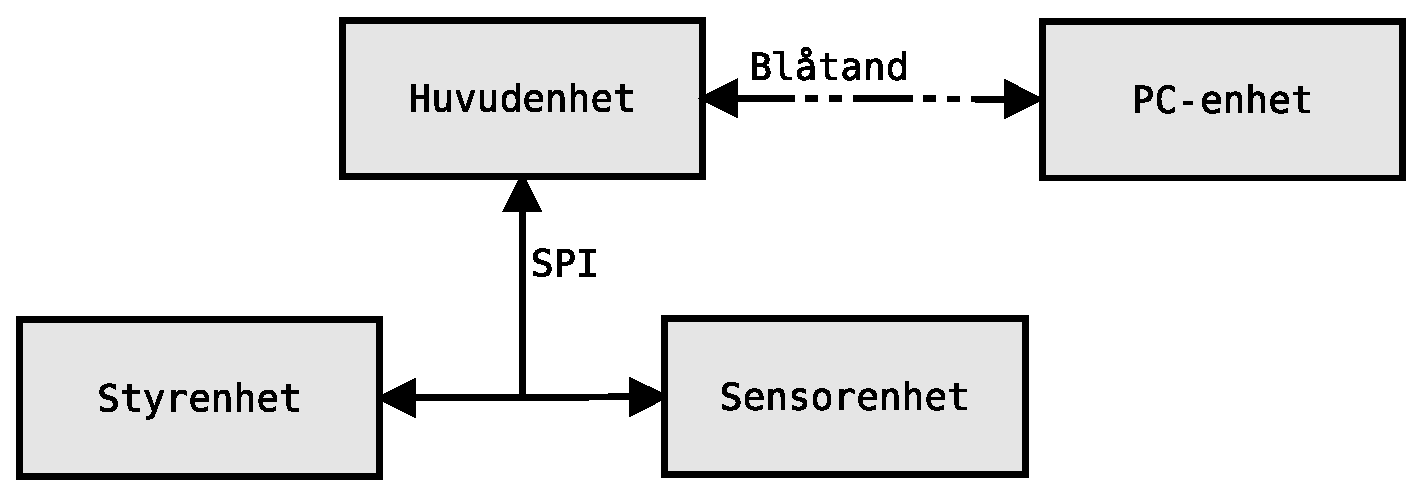
\includegraphics[scale=0.4]{grafik/kommunikation-oversikt}
	\caption{Översikt systemets kommunikationskanaler} \label{kommunikation-oversikt}
\end{figure}

Figur \ref{kommunikation-oversikt} ger en översikt av vilka moduler som kommunicerar med varandra och på vilket sätt detta sker. Styrenheten och Sensorenheten använder samma SPI-buss fast med olika Slave Select-pinnar. SPI-bussen körs på \todo{20kHz}.

\subsection{PCenhet $\longleftrightarrow$ Huvudenhet}

PC:n ansluter till Huvudenheten över ett Personal Area Network (PAN) via Blåtand. Alternativt kan en ethernetkabel eller ett trådlöst nätverk användas för att åstadkomma samma sak. Vi sätter sedan upp en TCP/IP-anslutning för att överföra information.

Kommunikation sker på initiativ av PCenheten. PCenheten skickar ett kommando till huvudenheten, och i det fall att det är status som begärs, svarar Huvudenheten. Kommandon ges i form av strängar, där en sträng kan innehålla godtyckligt många kommandon. Ett enskilt kommando ges på formen \texttt{kommando=argument1,argument2,...,argumentN}. Innehåller en sträng mer än ett kommando separeras varje kommando av semikolon.

När \texttt{status} begärs svarar huvudenheten på samma form som PCenheten med en sträng innehållandes relevant data separerade med semikolon. Tabell \ref{kommunikation-pc-huvud-status} listar vad och i vilken ordning Huvudenheten returnerar till PCenheten.

\begin{table}[h!]
	\centering
	\begin{tabularx}{\textwidth}{| l | X |}
		\hline
		\textbf{Attribut} & \textbf{Argument} \\\hline
	\end{tabularx}
	\caption{\todo{Lista precis vad status returnerar.}} \label{kommunikation-pc-huvud-status}
\end{table}

\subsubsection{Kommandon}

\begin{table}[h!]
	\centering
	\begin{tabularx}{\textwidth}{| l | l | X |}
		\hline
		\textbf{Instruktion} & \textbf{Argument} & \textbf{Beskrivning} \\\hline
		{autoMotor} & {True/False} & {Sätter motorerna till autonomt eller manuellt läge} \\\hline
		{autoArm} & {True/False} & {Sätter armen i autonomt eller manuellt läge} \\\hline
		{hasPackage} & {} & {Meddela roboten att vi har greppat ett paket} \\\hline
		{calibrateFloor} & {} & {Kalibrera sensorer efter golv} \\\hline
		{calibrateTape} & {} & {Kalibrera sensorer efter tejp} \\\hline
		{status} & {} & {Returnera robotens status} \\\hline
		{start} & {} & {Roboten påbörjar körning} \\\hline
		{armPosition} & {X,Y,Z,P,W,G} & {Förflytta armen till givna koordinater} \\\hline
		{motorSpeed} & {L,R} & {Sätt motorernas hastighet till givna hastigheter} \\\hline
	\end{tabularx}
	\caption{Kommandon från PCenhet till Huvudenhet} \label{protokoll:pc-huvud-tabell}
\end{table}

\subsection{Huvudenhet $\longleftrightarrow$ Styrenhet}

Huvudenheten kommunicerar med Styrenheten över SPI. Storleken på en instruktion är antingen fyra eller sju bytes lång. För att förebygga synkroniseringsproblem skickas först två startbytes bestående av hexadecimalt $0xff$ följt av längden på instruktionen (startbytesen och längdbyten räknas ej med). Därefter följer instruktionsbyten som består av två delar. De fyra högsta bitarna anger vilken instruktion som ska utföras enligt tabell \ref{protokoll:pc-motor-tabell}, och de fyra lägsta vilket servo eller motorpar instruktionen rör enligt tabell \ref{protokoll:pc-motor-adress-tabell}. I fallet att instruktionen är \texttt{Sätt register A till D} krävs dessutom två databytes.

Då ett motorpar adresseras anger den minsta biten i den första databyten vilken riktning motorparet skall röra sig. $0$ anger framåt, $1$ bakåt \todo{Stämmer?}. Den andra databyten anger vilken fart vi vill att motorerna skall röra sig i. Notera att motorernas hastighet sätts med instruktionen \texttt{Sätt register A till D}.

De servon vi arbetar med har en upplösning på 10 bitar både för position och hastighet. Vi måste alltså ha två databytes när vi vill ändra någon egenskap hos dessa. De två minsta bitarna i den första databyten är de två högsta bitarna och därefter följer den andra databyten.

\todo{Tabell för att illustrera bitar hit och dit?}

\subsection{Instruktionslista}

\begin{table}[h!]
	\centering
	\begin{tabularx}{\textwidth}{| l | l | X |}
		\hline
		\textbf{Instruktion} & \textbf{Argument} & \textbf{Beskrivning} \\\hline
		{0000} & {} & {Stoppa samtliga servon och motorer \todo{Behöver implementeras}} \\\hline
		{0001} & {A, D} & {Sätt register A till D} \\\hline
		{0010} & {A} & {Utför givna kommandon för A} \\\hline
		{0011} & {A, D} & {Sätt servohastighet för A till D} \\\hline
		{0100} & {A} & {Returnera Status för A \todo{Ska det användas? Isf vad returnerar det}} \\\hline
	\end{tabularx}
	\caption{Kommandon från huvudenhet till styrenhet \todo{Stämmer tabellen?}} \label{protokoll:pc-motor-tabell}
\end{table}

\begin{table}[h!]
	\centering
	\begin{tabularx}{\textwidth}{| l | X |}
		\hline
		\textbf{Adress} & \textbf{Beskrivning} \\\hline
		{0000} & {Höger hjulpar} \\\hline
		{0001} & {Vänster hjulpar} \\\hline
		{0010} & {Arm axel 1} \\\hline
		{0100} & {Arm axel 2} \\\hline
		{0110} & {Arm axel 3} \\\hline
		{1000} & {Arm axel 4} \\\hline
		{1011} & {Arm axel 5 (\textit{gripklo})} \\\hline
		{1100} & {Samtliga motorer} \\\hline
		{1101} & {Samtliga servon} \\\hline
		{1111} & {Samtliga motorer och servon} \\\hline
	\end{tabularx}
	\caption{Adresser för adressering till styrenhet} \label{protokoll:pc-motor-adress-tabell}
\end{table}

\subsection{Huvudenhet $\longleftrightarrow$ Sensorenhet}

Huvudenheten kommunicerar med Sensorenheten över SPI. Protokollet mellan dessa moduler är väldigt primitivt då det endast finns en instruktion, \texttt{Returnera sensordata för A}. Instruktionen anges av de fyra högsta bitarna av instruktionsbyten enligt tabell \ref{protokoll:huvud-sensor}. Huvudenhetens begäran är då bara på en enda databyte och Sensorenheten svarar omedelbart med de 8 högsta bitarna för den efterfrågade sensorn. Vilken sensor som enheten returnerar data för anges av de fyra minsta bitarna i instruktionsbyten enligt tabell \ref{protokoll:huvud-sensor-adress}.

\subsection{Instruktionslista}

\begin{table}[h!]
	\centering
	\begin{tabularx}{\textwidth}{| l | l | X |}
		\hline
		\textbf{Instruktion} & \textbf{Argument} & \textbf{Beskrivning} \\\hline
		{0000} & {A} & {Returnera sensordata för A} \\\hline
	\end{tabularx}
	\caption{Instruktion från huvudenhet till sensorenhet} \label{protokoll:huvud-sensor}
\end{table}

\begin{table}[h!]
	\centering
	\begin{tabularx}{\textwidth}{| l | X |}
		\hline
		\textbf{Adress} & \textbf{Beskrivning} \\\hline
		{0000} & {Linjesensor 1} \\\hline
		{0001} & {Linjesensor 2} \\\hline
		{0010} & {Linjesensor 3} \\\hline
		{0011} & {Linjesensor 4} \\\hline
		{0100} & {Linjesensor 5} \\\hline
		{0101} & {Linjesensor 6} \\\hline
		{0110} & {Linjesensor 7} \\\hline
		{0111} & {Linjesensor 8} \\\hline
		{1000} & {Linjesensor 9} \\\hline
		{1001} & {Linjesensor 10} \\\hline
		{1010} & {Linjesensor 11} \\\hline
		{1011} & {Avståndssensor Höger} \\\hline
		{1100} & {Avståndssensor Vänster} \\\hline
		{1101} & {Linjesensor center Vänster} \\\hline
		{1101} & {Linjesensor center Höger} \\\hline
	\end{tabularx}
	\caption{Adresser för instruktioner till sensorenhet} \label{protokoll:huvud-sensor-adress}
\end{table}
